\qquad
首先确保网络通畅,查看本机IPv4地址(调用Windows控制台ipconfig命令查看)和服务端IPv4地址(打开相应的网页,按F12查看),本实验中客户端地址为192.168.123.64,客户端处于一个子网中,服务端地址为202.117.1.185。\\
\qquad
在浏览器URL栏输入“https://cas.xjtu.edu.cn/login”,回车后打开西安交通大学学生版统一身份认证网关,如图 \ref{fig2} 所示。\\
\begin{figure}
	\centering
	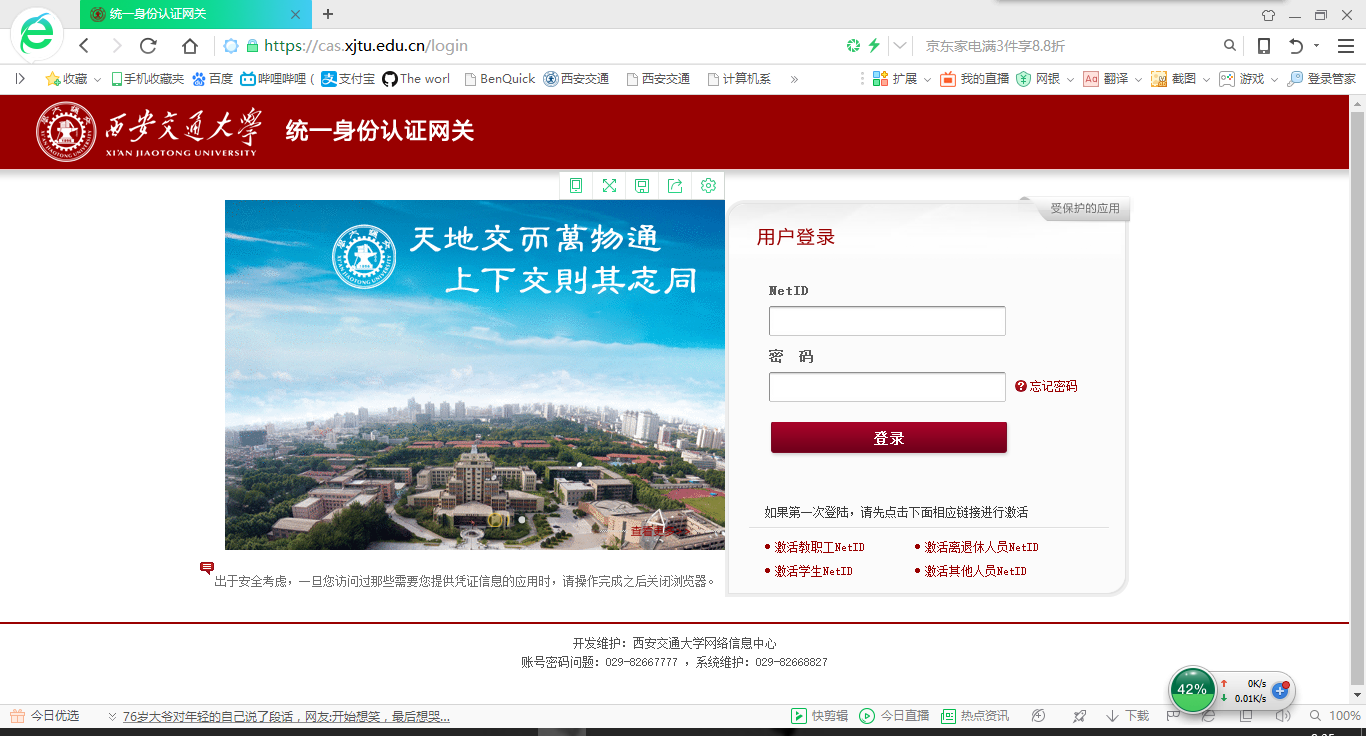
\includegraphics[width=12cm]{image/XJTU-Certificate}
	\caption{西安交通大学学生版统一身份认证网关}
	\label{fig2}
\end{figure}
\qquad
打开Wireshark软件,在初始界面选择活跃的网络连接,如图 \ref{fig3} 所示。本实验中客户端计算机通过无线局域网上网,所以选择WLAN连接。\\
\begin{figure}
	\centering
	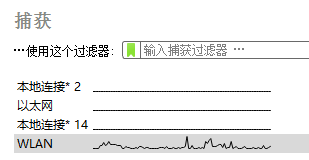
\includegraphics[width=8cm]{image/Wireshark-1}
	\caption{在Wireshark初始界面选择活跃的网络连接}
	\label{fig3}
\end{figure}
\qquad
在打开验证页面上输入用户名和密码,在点击登录之前,先确定Wireshark开始捕获分组,然后再进行登录。当页面上提示登陆成功后,停止捕获分组。将捕获到的分组保存为本地文件,以方便日后查看。本次实验中捕获到的分组如图 \ref{fig4} 所示。\\
\begin{figure}
	\centering
	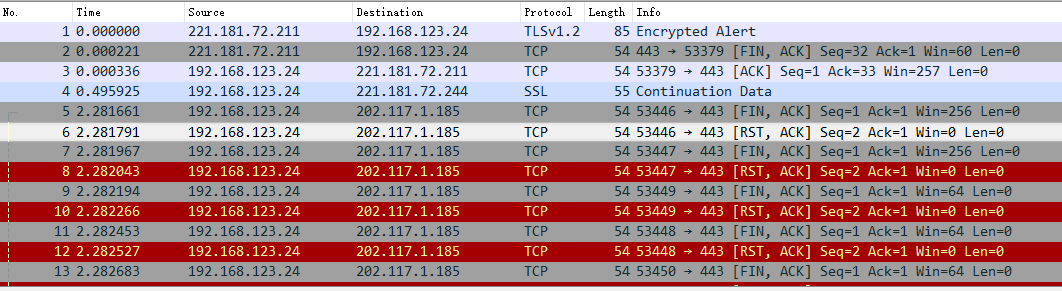
\includegraphics[width=12cm]{image/Wireshark-2}
	\caption{Wireshark捕获的分组(局部)}
	\label{fig4}
\end{figure}
\qquad
在图 \ref{fig4} 中,不同类型的分组用不同的颜色标出,可以通过点击“视图->着色规则”菜单项查看不同颜色所代表的的分组类型,如图 \ref{fig5} 所示。根据图 \ref{fig5} ,可以看到图 \ref{fig4} 捕获的分组中既包括UDP分组、TCP分组、TCP握手分组和TCP RST(复位)分组。其中,客户端(192.168.123.64)在与认证网关服务端(202.117.1.185)建立连接的过程中有多个RST分组(红色);产生RST的原因很多,不过根据图 \ref{fig4} 捕获的分组来看是由于服务端的443端口未被进程监听或被占用,而客户端又向服务端发送目标端口为443的连接请求,这时客户端则会发送RST分组以重新建立连接。\\
\begin{figure}
	\centering
	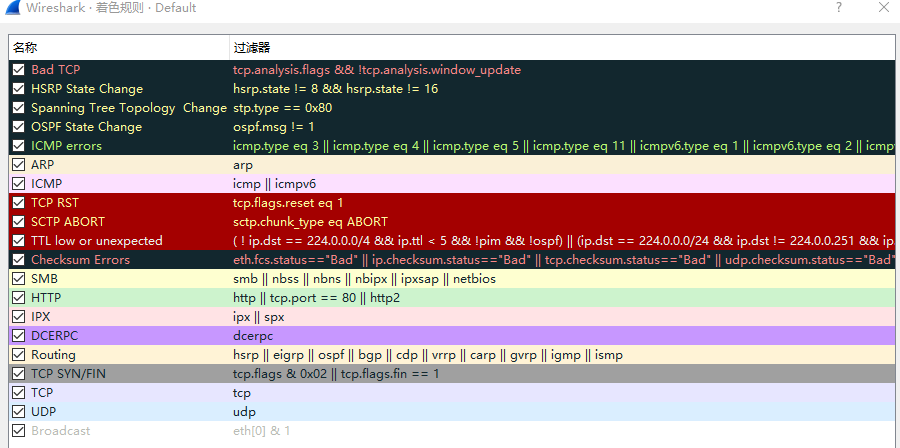
\includegraphics[width=12cm]{image/Wireshark-3}
	\caption{着色规则}
	\label{fig5}
\end{figure}